% !TEX root = ../my-thesis.tex
%
\chapter{The masses and dynamics of star clusters in the Milky Way}
\label{sec:dynamics}

\cleanchapterquote{Things are only impossible until they're not.}{Jean-Luc Picard}{(2364)}

\authorship{The results presented in this chapter will be published in Hunt and Reffert (\emph{in prep.}). All calculations, figures, and writing in this chapter were conducted by myself.}

\todo{dynamics section}

% -------------------------------------
\section{Introduction}
\label{sec:dynamics:introduction}

% PLAN
% - Masses are useful! Dynamics are useful! They're comparable to theory and represent measurements of fundamental (physical) parameters of OCs.
% - BUT: very limited measurements so far of these parameters.
% - Difficult to define OCs robustly without them (Hunt & Reffert 2023)
% - Empirical cuts on parameters insufficient to measure them.
% - MASSES: can be measured more or less two ways: counting stars or tidal parameters
% - discuss pros and cons of each way
% - DYNAMICS: some progress in studying for OCs in MW, but generally for small numbers of clusters only.
% - most clusters found to be supervirial. really?? what about as function of cluster mass, age, etc?
% - finally: masses useful for e.g. analysis of sample completeness. is a more fundamental physical parameter than the observed number of stars
% - give overview of what's in this chapter
% - emphasise that I'll be 


% -------------------------------------
\section{Mass calculations}
\label{sec:dynamics:masses}

% PLAN
% - give a quick overview of what's in this methods section


\subsection{Inference of stellar primary masses}
\label{sec:dynamics:masses:isochrones}

\begin{figure}[t]
    \centering
    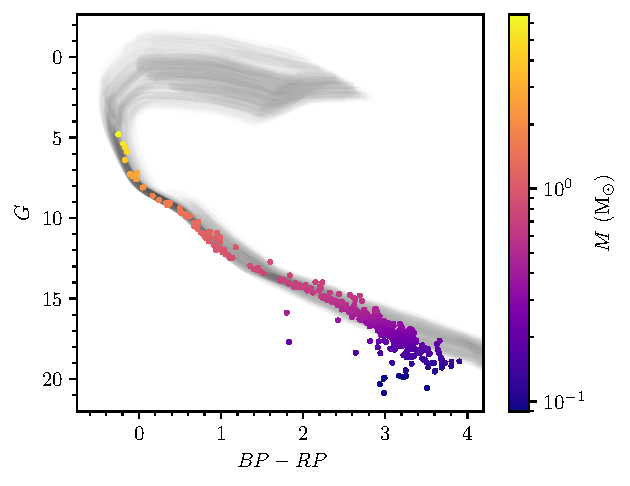
\includegraphics[width=0.8\textwidth]{fig/c4/masses_stellar.pdf}
    \caption[TODO]{TODO}
    \label{fig:dynamics:masses:stellar_masses}
 \end{figure}


\subsection{Correction for selection effects}
\label{sec:dynamics:masses:selection}

\begin{figure}[p]
    \centering
    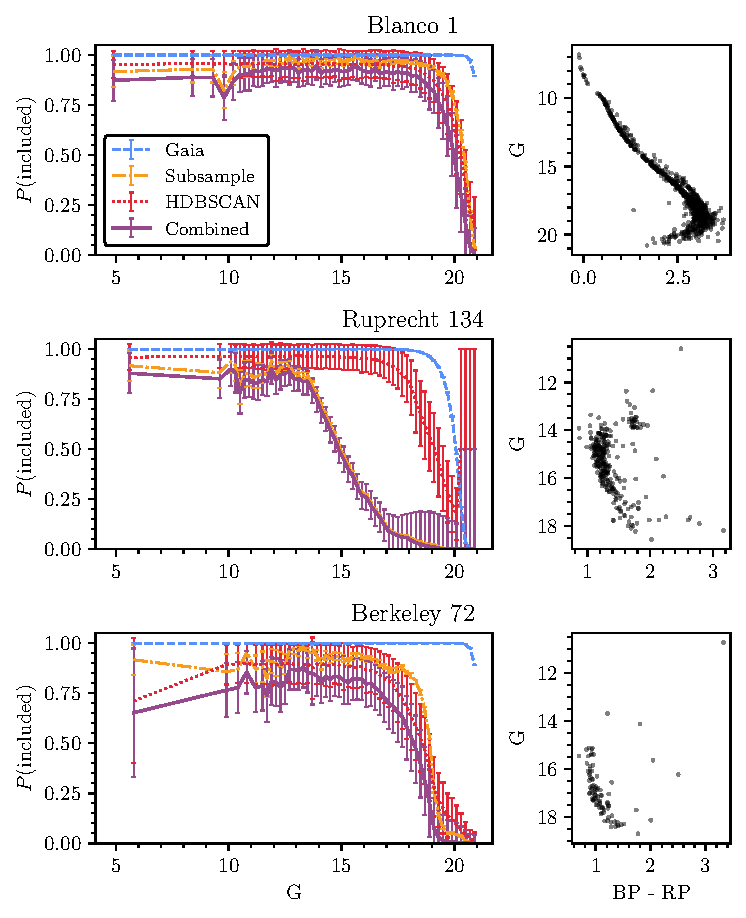
\includegraphics[width=\textwidth]{fig/c4/mass_selection_functions.pdf}
    \caption[TODO]{TODO}
    \label{fig:dynamics:masses:selection_effects}
 \end{figure}


\subsection{Correction for binaries}
\label{sec:dynamics:masses:binaries}


\subsection{Mass function fits}
\label{sec:dynamics:masses:imf_fits}

\begin{figure}[p]
    \centering
    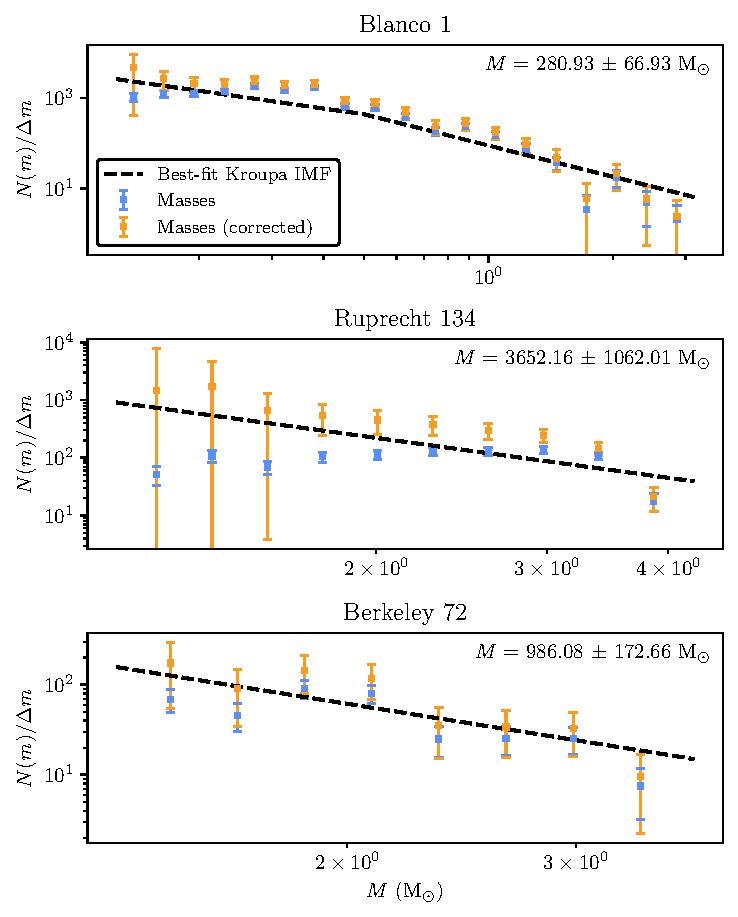
\includegraphics[width=\textwidth]{fig/c4/mass_functions.pdf}
    \caption[TODO]{TODO}
    \label{fig:dynamics:masses:mass_functions}
 \end{figure}


\subsection{Jacobi radius inference}
\label{sec:dynamics:masses:jacobi}

\begin{figure}[t]
    \centering
    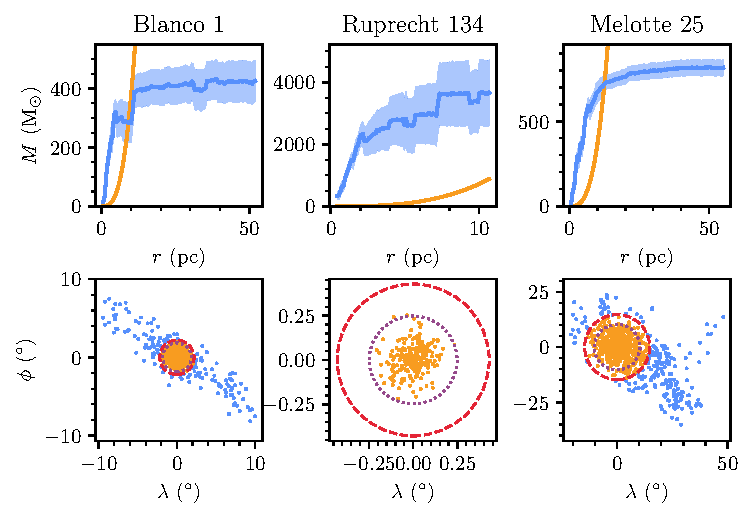
\includegraphics[width=\textwidth]{fig/c4/masses_jacobi_radii.pdf}
    \caption[TODO]{TODO}
    \label{fig:dynamics:masses:radii}
 \end{figure}



% -------------------------------------
\section{Velocity dispersion inference}
\label{sec:dynamics:velocities}


\subsection{Gaussian velocity dispersion model}
\label{sec:dynamics:velocities:model}


\subsection{Coordinate frame and radial velocity corrections}
\label{sec:dynamics:velocities:correction}


\subsection{Binary star contamination}
\label{sec:dynamics:velocities:binaries}

\begin{figure}[t]
    \centering
    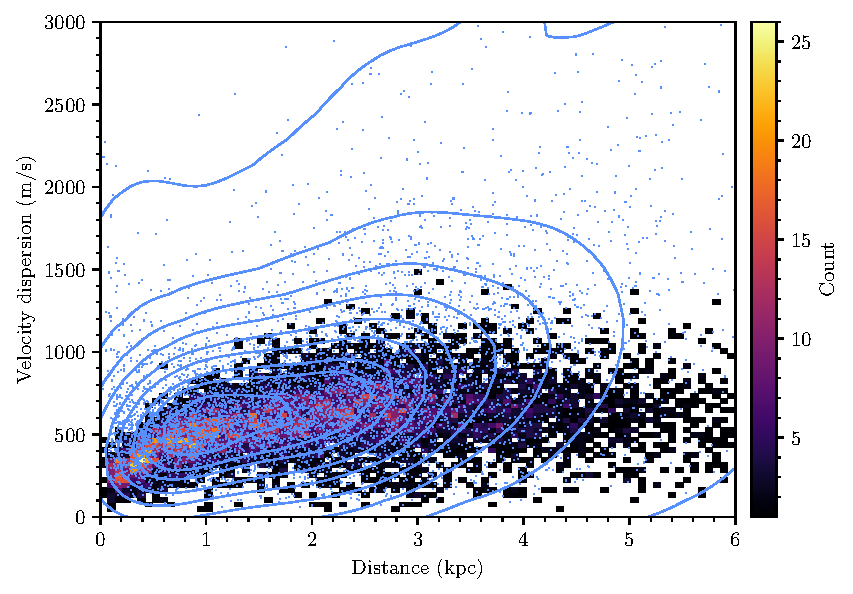
\includegraphics[width=\textwidth]{fig/c4/dispersion_binaries.pdf}
    \caption[TODO]{TODO}
    \label{fig:dynamics:velocities:binary_contamination}
 \end{figure}


% -------------------------------------
\section{Results}
\label{sec:dynamics:results}


\subsection{Masses}
\label{sec:dynamics:results:masses}

\begin{figure}[t]
    \centering
    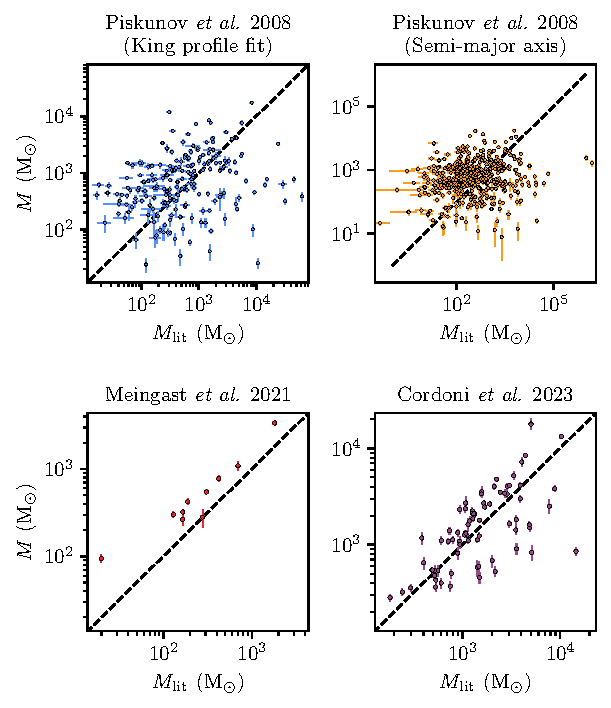
\includegraphics[width=\textwidth]{fig/c4/results_mass_comparison.pdf}
    \caption[TODO]{TODO}
    \label{fig:dynamics:results:mass_comparison}
 \end{figure}


\subsection{Jacobi radii}
\label{sec:dynamics:results:radii}

\begin{figure}[t]
    \centering
    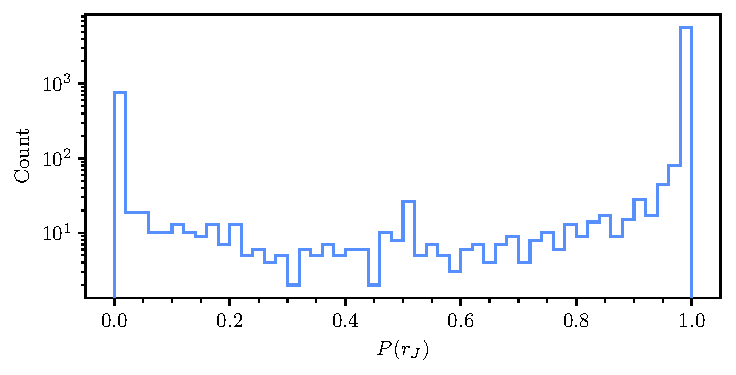
\includegraphics[width=\textwidth]{fig/c4/results_p_jac_distribution.pdf}
    \caption[TODO]{TODO}
    \label{fig:dynamics:results:jacobi_radii_distribution}
 \end{figure}


\subsection{Virial ratios}
\label{sec:dynamics:results:virial}

\begin{figure}[t]
    \centering
    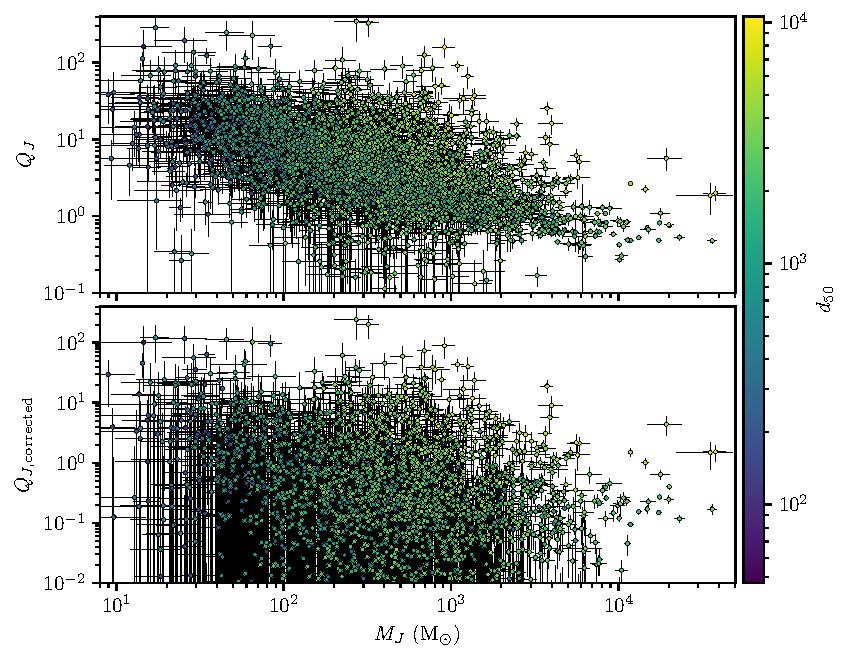
\includegraphics[width=\textwidth]{fig/c4/results_virial_vs_mass.pdf}
    \caption[TODO]{TODO}
    \label{fig:dynamics:results:virial_vs_mass}
 \end{figure}

\begin{figure}[t]
    \centering
    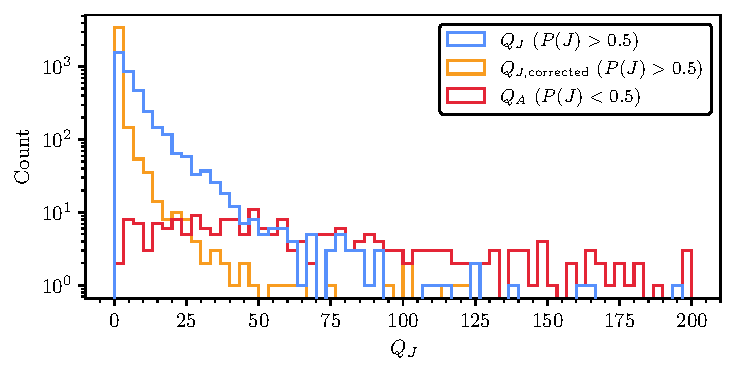
\includegraphics[width=\textwidth]{fig/c4/results_q_distribution.pdf}
    \caption[TODO]{TODO}
    \label{fig:dynamics:results:virial_ratio_distribution}
 \end{figure}


\subsection{An updated observational definition of open clusters}
\label{sec:dynamics:results:definition}

\begin{table}[t]

% Define first header
\caption{\label{tab:dynamics:catalogue_results}TODO}

\centering
\begin{tabular}{lcc}
\hline\hline
Type & Identifier & Count \\
\hline

OC & \texttt{o} & TODO \\
- bound OC & \texttt{o} & TODO \\
- unbound OC & \texttt{ou} & TODO \\
\hline
MG & \texttt{m} & TODO \\
- $P(r_J) < 0.5$ & \texttt{m} & TODO \\
- $P(r_J) > 0.5$, $M_J < 50$ \MSun & \texttt{mj} & TODO \\
\hline
GC & \texttt{g} & TODO \\

\end{tabular}

% \tablefoot{
% \tablefoottext{a}{}
% }

\end{table}    


% -------------------------------------
\section{Discussion}
\label{sec:dynamics:discussion}


\subsection{Completeness of the \gaia\ DR3 open cluster census}
\label{sec:dynamics:results:completeness}


% -------------------------------------
\section{Conclusions and areas for improvement before publication}
\label{sec:dynamics:conclusion}
